\documentclass[a11paper]{article}

\usepackage{karnaugh-map}
\usepackage{subcaption}
\usepackage{tabularx}
\usepackage{libs/titlepage}
\usepackage{libs/document}
\usepackage{booktabs}
\usepackage{multicol}
\usepackage{float}
\usepackage{varwidth}
\usepackage{graphicx}
\usepackage{siunitx}
% \usepackage[toc,page]{appendix}
\usepackage[usenames,dvipsnames]{xcolor}

\title{Rapport d'APP}

\class{Logique Combinatoire}
\classnb{GEN420 \& GEN430}

\teacher{Marwan Besrour \& Gabriel Bélanger}

\author{
  \addtolength{\tabcolsep}{-0.4em}
  \begin{tabular}{rcl} % Ajouter des auteurs au besoin
      Benjamin Chausse & -- & CHAB1704 \\
      Shawn Couture    & -- & COUS1912 \\
  \end{tabular}
}

\newcommand{\todo}[1]{\begin{color}{Red}\textbf{TODO:} #1\end{color}}
\newcommand{\note}[1]{\begin{color}{Orange}\textbf{NOTE:} #1\end{color}}
\newcommand{\fixme}[1]{\begin{color}{Fuchsia}\textbf{FIXME:} #1\end{color}}
\newcommand{\question}[1]{\begin{color}{ForestGreen}\textbf{QUESTION:} #1\end{color}}

\begin{document}
\maketitle
\newpage
\tableofcontents
\newpage

\section{Module \texttt{thermo2bin}}
\subsection{Démarche et équations}

L’objectif était de convertir un code thermométrique de 12 bits en un code
binaire non signé sur 4 bits. Le nombre représenté par un tel code est obtenu
en comptant le nombre de bits à 1. Les équations logiques doivent donc
effectuer ce comptage. Étant donné que le code est sur 12 bits, il a été
divisé en trois groupes de 4 bits, ce qui a permis l'utilisation de tables de
Karnaugh pour déterminer les équations logiques.

D'après la table de vérité du code thermométrique 4 bits
(\ref{tab:table-de-vérité-thermométrique-4-bits}), le bit le plus
significatif du résultat binaire n’est jamais à 1. L'équation du bit $E$ est
donc simplement $E = 0$. Le bit $F$ est à 1 uniquement si $A$ l’est
également, d’où l’équation $F = A$. Les tables de Karnaugh ont donc été
utilisées uniquement pour les deux bits restants. Les deux tables, une pour
chaque bit, se trouvent en annexe (\ref{tab:karnaugh-bit-G} et
\ref{tab:karnaugh-bit-H}). Les équations étant assez simple, aucune simplification d'équations était nécessaire.

\begin{align}
	E & = 0         \\
	F & = A         \\
	G & = A'C       \\
	H & = C'D + A'B
\end{align}

Les trois résultats binaires sont ensuite additionnés à l’aide d’un
additionneur 4 bits, afin d’obtenir la valeur totale correspondant au nombre
de bits à 1 dans le code thermométrique. En ce qui concerne la détection
d'erreurs, une vérification par groupe de 2 bits est effectuée. Celle-ci
s’assure que, pour chaque paire consécutive, le LSB n’est pas à 0 si le MSB
est à 1, ce qui permet une détection rapide d’erreurs éventuelles (voir le
code en annexe).

\subsection{Explication des schémas blocs}

Le module \texttt{thermo2bin} est constitué de deux additionneurs 4 bits,
chacun composé de quatre additionneurs 1 bit. Les additionneurs 1 bit ont été
implémentés à l’aide de logique combinatoire ainsi que de blocs utilisant des
instructions \texttt{case}. Le module thermométrique comprend trois sections
identiques effectuant la conversion d’un code thermométrique 4 bits en un
code binaire non signé. Il intègre également une section de détection
d’erreurs, qui agit directement sur l’entrée du module. Il est à noter que
Vivado optimise certains sous-modules à l’aide de tables de correspondance
(\textit{look-up tables}) afin d’améliorer leur performance par rapport à une
implémentation reposant uniquement sur des portes logiques élémentaires.

\subsection{Fréquence d’opération}

Pour déterminer la fréquence d’opération maximale, il faut analyser le schéma
obtenu lorsque tout les sous-modules sont combinés et identifier le chemin le
plus long qu’un signal peut parcourir de l’entrée à la sortie. Cette analyse
peut être effectuée en observant les schémas générés par Vivado.

Le chemin le plus long à l’intérieur d’un additionneur 1 bit se situe entre
les bits d’entrée et le signal de retenue (\textit{carry-out}), ce qui
représente un total de 3 portes logiques dans le premier additionneur 1 bit.
Par la suite, les additionneurs 1 bit sont chaînés via les signaux
\textit{carry-in} et \textit{carry-out}, avec 2 portes logiques
supplémentaires par liaison. Un additionneur 4 bits utilise ainsi 4
additionneurs 1 bit en série, ce qui donne un chemin critique de
$2 \times 4 + 1 = 9$ portes logiques.

Le module \texttt{thermo2bin} contient deux additionneurs 4 bits chaînés. Le
second additionneur reçoit en entrée le \textit{carry-out} du premier,
ajoutant 8 portes logiques supplémentaires. Le total pour les deux blocs est
donc d’environ 17 portes logiques. Du côté des entrées, le bit le plus
coûteux en logique est $H$, avec le chemin suivant : $C' \rightarrow (C'D)
	\rightarrow (C'D + A'B)$, soit 3 portes logiques supplémentaires. On obtient
ainsi un total d’environ 20 portes logiques.

En supposant un temps de propagation de $5,\text{ns}$ par porte, le temps de
propagation maximal est donc approximativement $20 \times 5 = 100,\text{ns}$.
Sans tenir compte du temps de lecture ni des \textit{buffers} que Vivado
pourrait ajouter aux entrées et sorties, la fréquence maximale estimée est :

\begin{align}
	\frac{1}{100 \times 10^{-9}} & \approx \SI{10}{\mega\hertz}
\end{align}

Ce résultat est loin des $20,\text{MHz}$ exigés. Cependant, Vivado optimise
les additionneurs 1 bit à l’aide de \textit{look-up tables}, réduisant le
circuit logique de 3 à 1 porte logique dans certains cas. Cela abaisse le
nombre total de portes logiques à environ 11, ce qui améliore la fréquence
maximale à:

\begin{align}
	\frac{1}{11 \times 5 \times 10^{-9}} & \approx \SI{18.18}{\mega\hertz}
\end{align}

Ce n’est toujours pas suffisant pour atteindre l’objectif fixé.

\subsection{Implémentation}

Le code VHDL du module \texttt{thermo2bin} est fourni en annexe. Trois
composantes sont utilisées de façon hiérarchique. Le module principal aurait
pu être divisé en sous-modules de 4 bits, mais pour des raisons
d’optimisation, les trois conversions de segments de 4 bits du vecteur
thermométrique de 12 bits sont intégrées dans un seul bloc.

Après l’instruction \texttt{begin}, on retrouve trois sections quasi
identiques effectuant les équations booléennes de conversion. Les résultats
sont stockés dans trois signaux intermédiaires, lesquels sont additionnés
séquentiellement à l’aide d’additionneurs 4 bits. Le résultat du premier et
du deuxième segment est additionné, puis le résultat est additionné au
troisième segment. Un signal de retenue (\textit{carry}) permet la liaison
entre les deux additionneurs. Le résultat final est assigné à la sortie du
module \texttt{thermo2bin}. La logique de détection d’erreur est placée à la
fin du code et a été expliquée dans la section sur la démarche.

Le code VHDL de l’additionneur 4 bits est simple : quatre instances de
l’additionneur 1 bit y sont instanciées. Des signaux intermédiaires assurent
la propagation du \textit{carry} d’un bloc à l’autre ainsi que la
transmission des bits à additionner à chaque position. Le premier
additionneur traite les bits de poids faible (\textit{LSB}) et transmet le
\textit{carry} au suivant, qui additionne les bits de poids 1, et ainsi de
suite.

Les additionneurs 1 bit sont eux aussi simples : ils sont issus d’une table
de vérité à partir de laquelle une expression booléenne a été dérivée.

\section{Simulation complète}

Tous les modules du projet possèdent leur propre banc de test, couvrant leurs
cas d’utilisation de manière unitaire. Par conséquent, le banc de test de
\texttt{AppCombiTop} ne reprend pas l’ensemble des tests du module 7
segments. Il vérifie que les boutons modifient les deux DELs de parité et que
l’entrée \texttt{ADCth} modifie les DELs PMOD.

Le banc de test de \texttt{thermo2bin} couvre tous les cas valides, ainsi que
quelques cas invalides. Les autres bancs de test valident les modules de
manière individuelle pour tous — ou presque tous — les cas pertinents. Il
aurait donc été redondant et inutilement long de dupliquer ces tests
unitaires dans \texttt{AppCombiTop}.

Le banc de test du \texttt{Mux} ne couvre pas toutes les combinaisons
possibles. Étant donné qu’il est composé de trois sous-modules ayant chacun
leur propre banc de test, cela aurait engendré une duplication inutile. Le
test se concentre sur les combinaisons de boutons causant une erreur, vérifie
que l’erreur est bien transmise à l’affichage 7 segments, que l’erreur en
entrée est bien gérée, et que toutes les combinaisons valides produisent la
bonne valeur affichée. Il vérifie aussi la présence du \texttt{Moins 5} sur
la sortie signée.

Il n’est pas nécessaire que le test de \texttt{thermo2bin} couvre les
$2^{12}$ combinaisons possibles. Il suffit de tester les 12 cas valides, de
vérifier la détection d’erreur sur toutes les paires de 2 bits, puis de
réaliser quelques tests aléatoires avec des zéros pour confirmer le bon
fonctionnement général.


Les bancs de test utilisent des instructions \texttt{assert} permettant
d’afficher dans le terminal si une divergence entre le résultat obtenu et le
résultat attendu survient. La majorité fonctionnent correctement, mais
certains rencontrent des problèmes liés aux valeurs indéfinies (\texttt{'U'})
entraînant des messages incohérents comme : "Obtenu 0, Voulu 0".
Malgré un débogage approfondi et un fonctionnement correct du module en
simulation, le banc de test du \texttt{Mux} présente encore des incohérences
dans les transitions, rendant les résultats difficiles à interpréter. Le
numéro de chaque test est donc indiqué directement sur son chronogramme.
Pour le banc de test de parité, deux chronogrammes sont fournis,
correspondant chacun à un état différent du bouton de configuration
(\texttt{cfg}). Certains tests présentent des problèmes de valeurs initiales,
comme des sorties changeant d'état sans modification des entrées. La
méthodologie utilisée pour concevoir les bancs de tests devra être revue pour
mitiger ces erreurs et clarifier les chronogrammes.
Tous les bancs de test incluent des valeurs \texttt{expected} pour les
sorties attendues. Les noms des signaux sont choisis pour refléter la
fonctionnalité du module testé, et non nécessairement le nom des signaux
internes de plus haut niveau.

\section{Démarche d'analyse de compatibilité}

La première étape a été d'analyser le signal d'entrée de la carte
thermométrique. La DEL 2 est connectée au connecteur \texttt{JD1} en
configuration \textit{pull-up}, ce qui signifie qu'un niveau logique bas
(\texttt{0}) est requis pour l'allumer.

Cependant, trois inverseurs sont connectés en série avant elle : deux
\texttt{74V1T04STR} et un \texttt{NC7SP04P5X}, alimentés à \SI{1.2}{V}. Après
analyse des seuils $V_{OH}$, $V_{OL}$, $V_{IH}$ et $V_{IL}$ des composants :

% La premiere etape a ete d'analy

\begin{itemize}
	\item Le \texttt{NC7SP04P5X} produit un $V_{OH}$ maximal de \SI{1.1}{V} ;
	\item Le \texttt{74V1T04STR} requiert un $V_{IH}$ minimal de \SI{2.0}{V}.
\end{itemize}

Cela implique que le signal en sortie du \texttt{NC7SP04P5X} est toujours
considéré comme un niveau bas par le \texttt{74V1T04STR}. En conséquence, la
DEL reste allumée en permanence, sauf lorsque le connecteur de test force un
niveau haut adéquat à l’entrée des \texttt{74V1T04STR}.

\newpage
\appendix
\begin{figure}[H]
  \centering
	\begin{subfigure}{.496\linewidth}
		\centering
		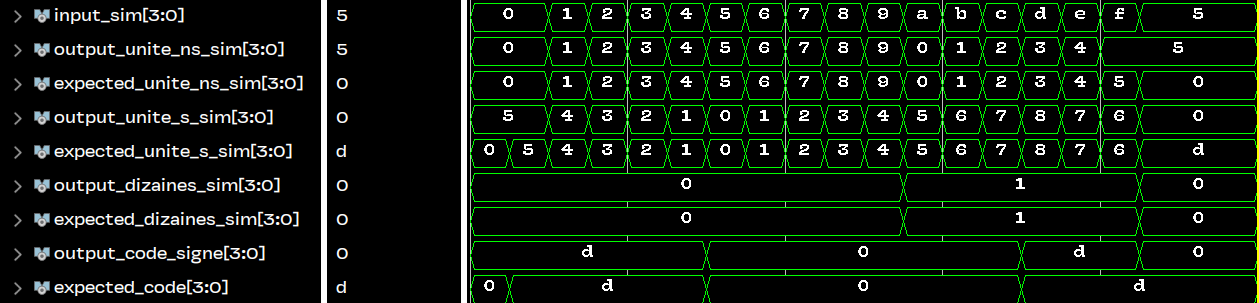
\includegraphics[width=\textwidth]{figures/img/graph-bin2dualbcd.png}
		\caption{Bin2DualBCD}
	\end{subfigure}
	\begin{subfigure}{.496\linewidth}
		\centering
		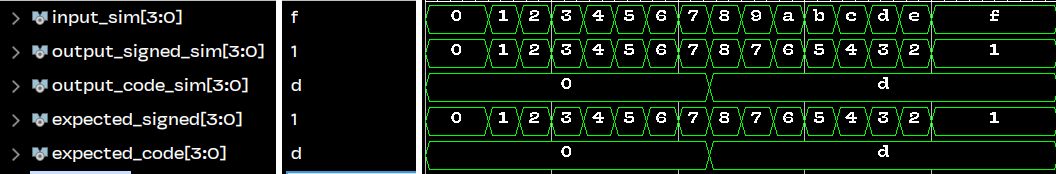
\includegraphics[width=\textwidth]{figures/img/graph-bin2dualbcd-signed.png}
		\caption{graph-bin2dualbcd-signed}
	\end{subfigure}
	\begin{subfigure}{.496\linewidth}
		\centering
		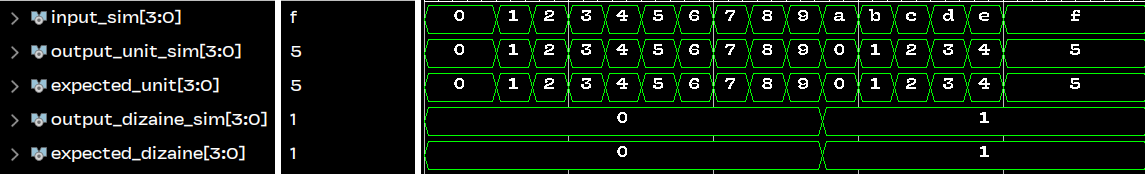
\includegraphics[width=\textwidth]{figures/img/graph-bin2dualbcd-unsigned.png}
		\caption{graph-bin2dualbcd-unsigned}
	\end{subfigure}
	\begin{subfigure}{.496\linewidth}
		\centering
		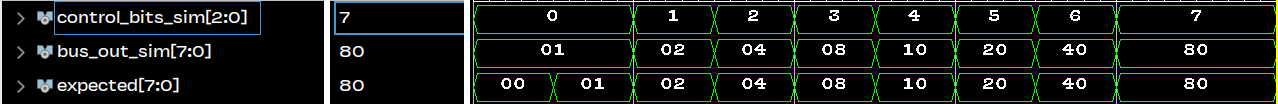
\includegraphics[width=\textwidth]{figures/img/graph-dec-2-a-8.png}
		\caption{graph-dec-2-a-8}
	\end{subfigure}
	\begin{subfigure}{.496\linewidth}
		\centering
		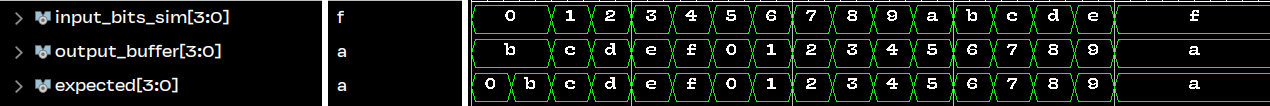
\includegraphics[width=\textwidth]{figures/img/graph-moins5.png}
		\caption{graph-moins5}
	\end{subfigure}
	\begin{subfigure}{.496\linewidth}
		\centering
		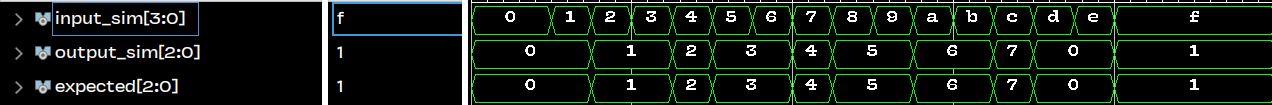
\includegraphics[width=\textwidth]{figures/img/graph-mult-2-3.png}
		\caption{graph-mult-2-3}
	\end{subfigure}
	\begin{subfigure}{.496\linewidth}
		\centering
		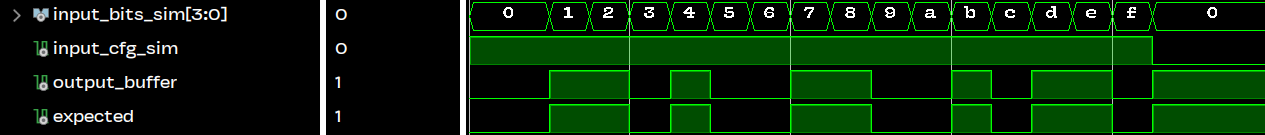
\includegraphics[width=\textwidth]{figures/img/graph-parite-pressed.png}
		\caption{graph-parite-pressed}
	\end{subfigure}
	\begin{subfigure}{.496\linewidth}
		\centering
		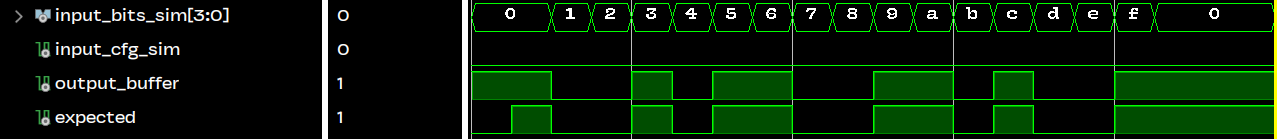
\includegraphics[width=\textwidth]{figures/img/graph-parite-unpressed.png}
		\caption{graph-parite-unpressed}
	\end{subfigure}
	\begin{subfigure}{.49\linewidth}
		\centering
		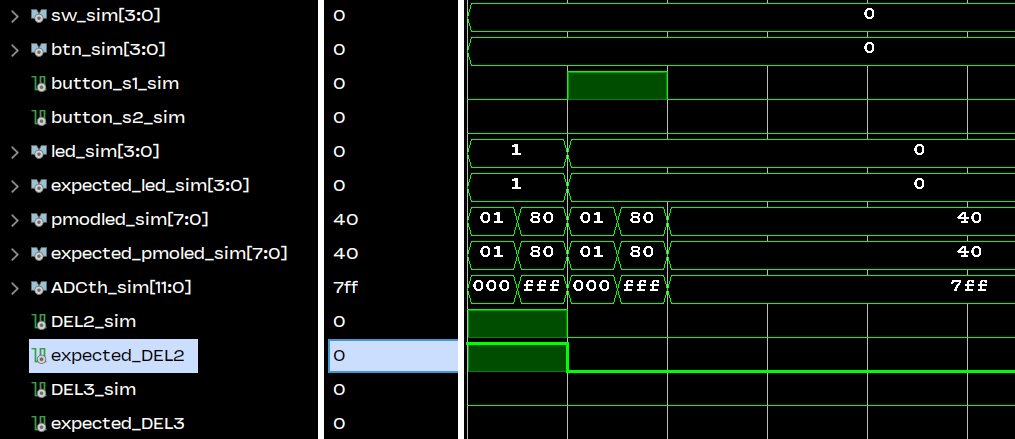
\includegraphics[width=\textwidth]{figures/img/graph-appcombitop.png}
		\caption{graph-appcombitop}
	\end{subfigure}
	\begin{subfigure}{.496\linewidth}
		\centering
		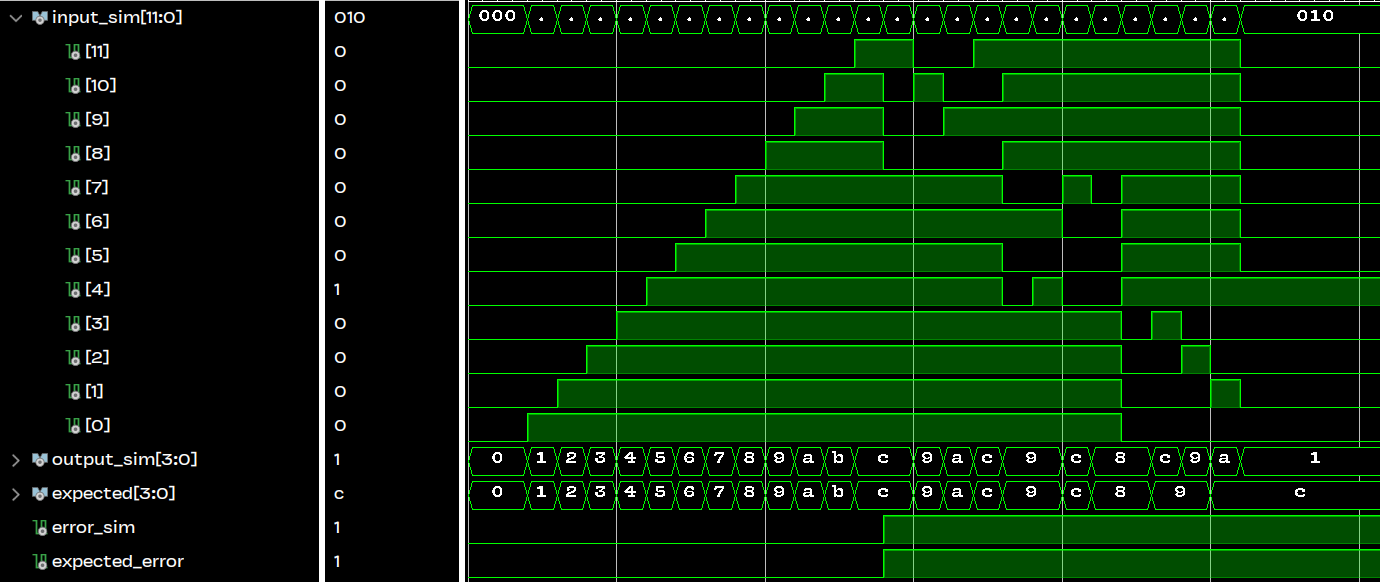
\includegraphics[width=\textwidth]{figures/img/graph-thermo2bin.png}
		\caption{graph-thermo2bin}
	\end{subfigure}
	\begin{subfigure}{.496\linewidth}
		\centering
		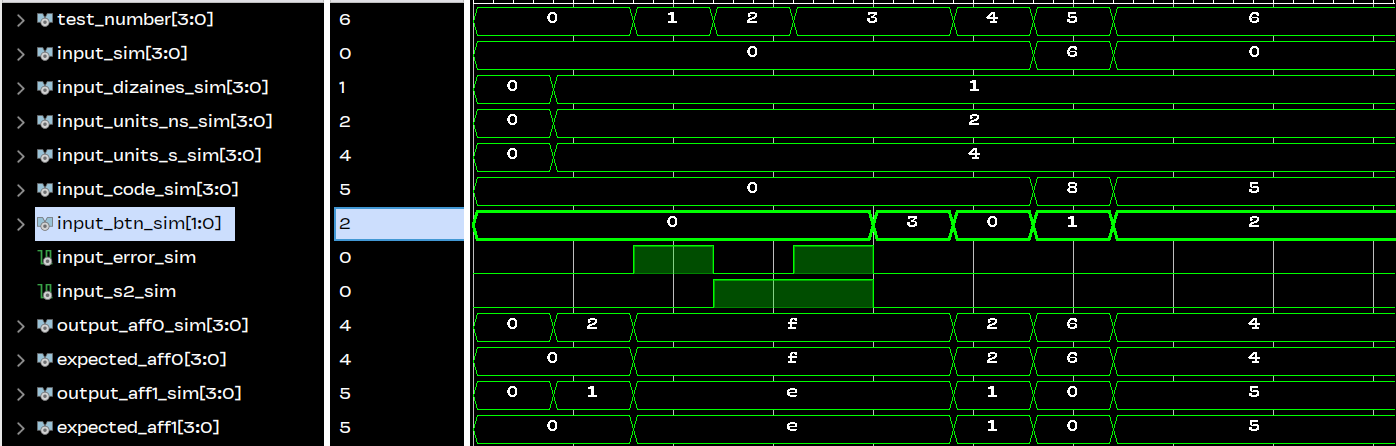
\includegraphics[width=\textwidth]{figures/img/graph-mux.png}
		\caption{graph-mux}
	\end{subfigure}
	\caption{Chronogrames des simulations Vivado}
\end{figure}



\section{Code VHDL}

\begin{figure}[H]
	\tiny
	\centering
	\begin{varwidth}{\linewidth}
		\input{figures/code/thermo2bin.tex}
	\end{varwidth}
	\caption{Module Thermo2bin}
\end{figure}

\begin{figure}[H]
	\tiny
	\centering
	\begin{varwidth}{\linewidth}
		\input{figures/code/add4bits.tex}
	\end{varwidth}
	\caption{Module Add4Bits}
\end{figure}

\begin{figure}[H]
	\tiny
	\centering
	\begin{varwidth}{\linewidth}
		\input{figures/code/add1bita.tex}
	\end{varwidth}
	\caption{Module Add1BitA}
\end{figure}

\begin{figure}[H]
	\tiny
	\centering
	\begin{varwidth}{\linewidth}
		\input{figures/code/add1bitb.tex}
	\end{varwidth}
	\caption{Module Add1BitB}
\end{figure}

\section{Schémas Bloc}

\begin{figure}[H]
	\centering
	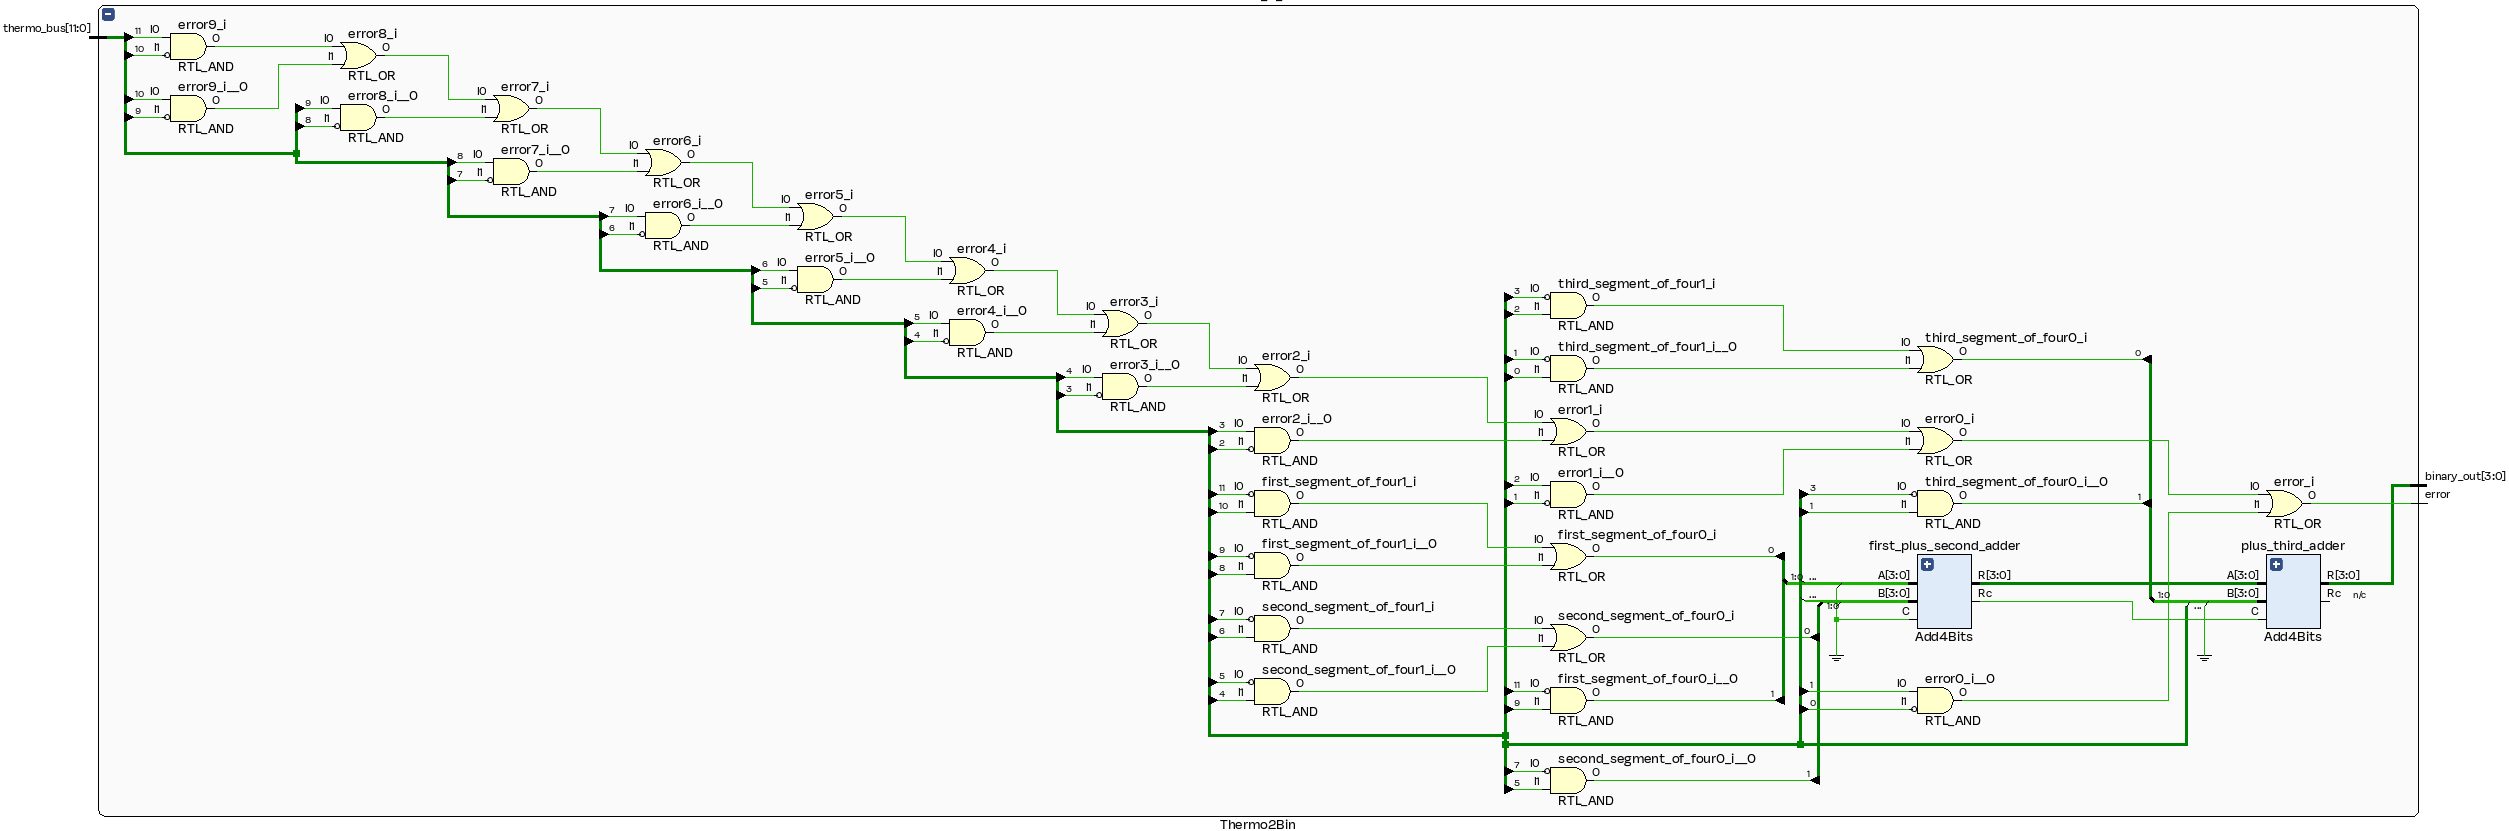
\includegraphics[width=\textwidth]{figures/img/schematic-thermo2bin.png}
	\caption{Module Thermo2bin}
\end{figure}

\begin{figure}[H]
	\centering
	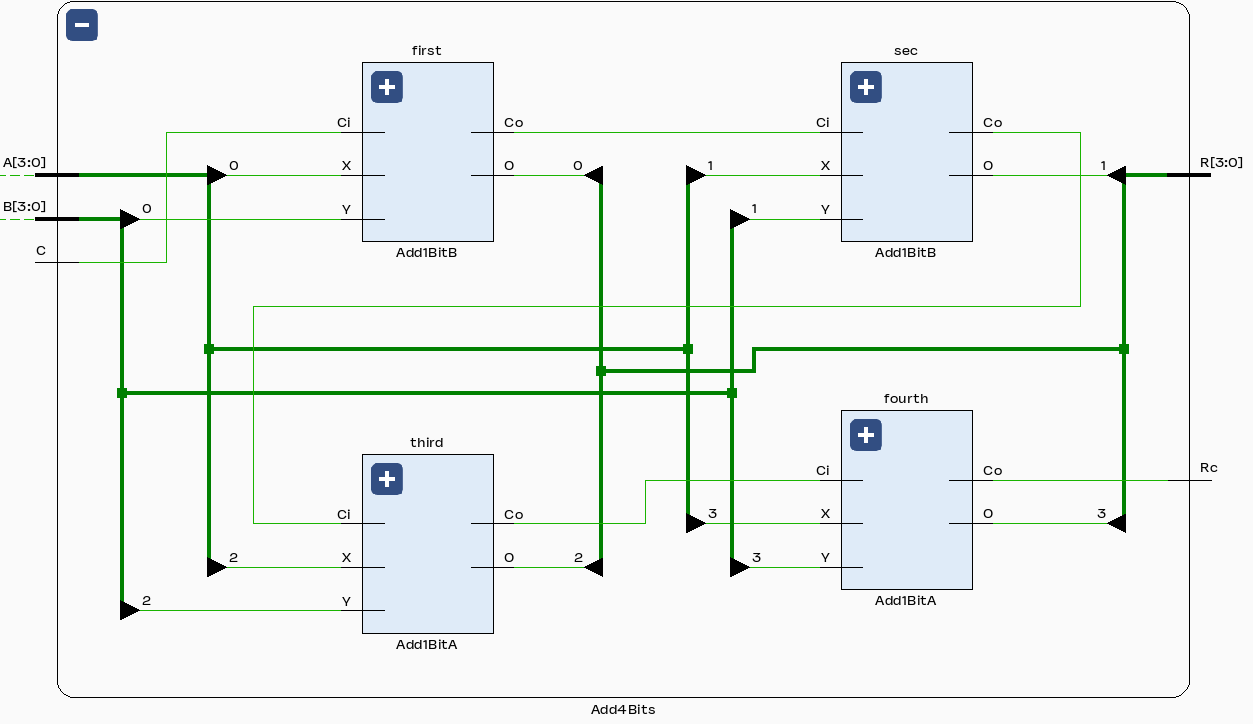
\includegraphics[width=.6\textwidth]{figures/img/schematic-add4bits.png}
	\caption{Module Add4Bits}
\end{figure}

\begin{figure}[H]
	\centering
	\begin{subfigure}{0.60 \linewidth}
		\centering
		\vfill
		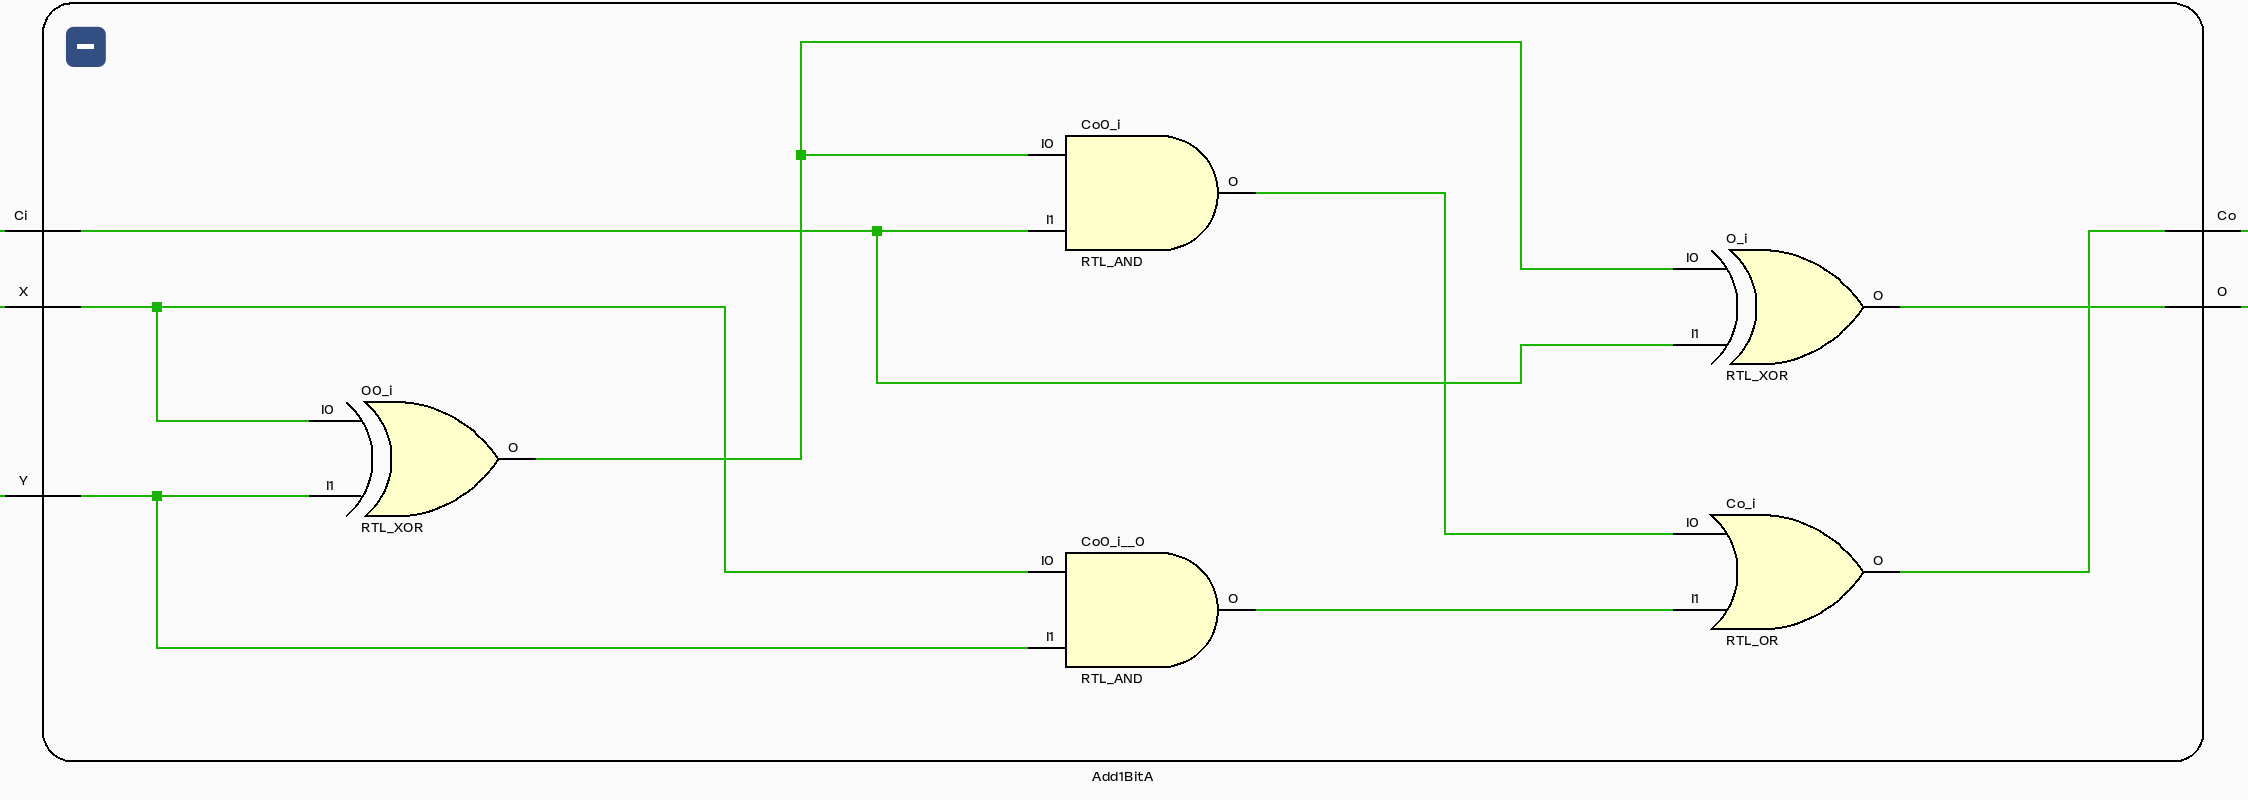
\includegraphics[width=\textwidth]{figures/img/schematic-add1bita.png}
		\caption{Add1BitA: Conception parallèle}
	\end{subfigure} \hfill
	\begin{subfigure}{0.39 \linewidth}
		\centering
		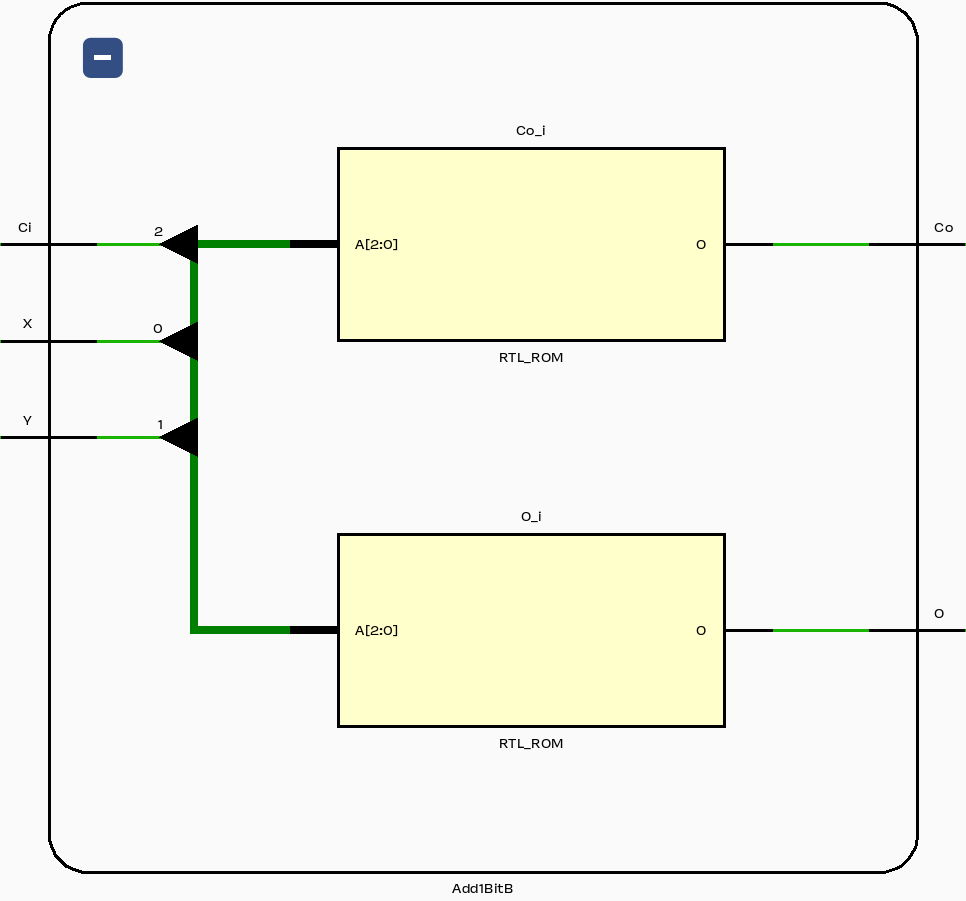
\includegraphics[width=\textwidth]{figures/img/schematic-add1bitb.png}
		\caption{Conception séquentielle avec \textit{CASE}}
	\end{subfigure}
	\caption{Additionneurs 1 bit}
\end{figure}


\section{Tables de Vérité et Karnaugh}

\begin{table}[H]
	\centering
	\caption{Table de vérité des Bits}
	\label{tab:table-de-vérité-thermométrique-4-bits}
	\vspace{.2cm}
	\begin{tabular}{llllllll}
		\toprule
		A & B & C & D & E & F & G & H \\
		\midrule
		0 & 0 & 0 & 0 & 0 & 0 & 0 & 0 \\
		0 & 0 & 0 & 1 & 0 & 0 & 0 & 1 \\
		0 & 0 & 1 & 1 & 0 & 0 & 1 & 0 \\
		0 & 1 & 1 & 1 & 0 & 0 & 1 & 1 \\
		1 & 1 & 1 & 1 & 0 & 1 & 0 & 0 \\
		\bottomrule
	\end{tabular}

\end{table}

% \begin{figure}[H]
% \centering
% \begin{karnaugh-map}[4][4][1][$D$][$C$][$B$][$A$]
% \manualterms{
%   0,1,2,3,
%   4,5,6,7,
%   8,9,10,11,
%   12,13,14,15
% }
% \implicant{1}{9}
% \implicant{4}{6}
% \end{karnaugh-map}
% \caption{Karnaugh pour le bit $H$}
% \end{figure}
%
\begin{figure}[H]
\centering
\begin{karnaugh-map}[4][4][1][$D$][$C$][$B$][$A$]
\manualterms{
	0,1,X,0,
	X,X,X,1,
	X,X,X,X,
	X,X,X,0}
\implicant{1}{9}
\implicant{4}{6}
\end{karnaugh-map}
\caption{Karnaugh pour le bit $H$}
\label{tab:karnaugh-bit-H}
\end{figure}

\begin{figure}[H]
\centering
\begin{karnaugh-map}[4][4][1][$D$][$C$][$B$][$A$]
\manualterms{
	0,0,X,1,
	X,X,X,1,
	X,X,X,X,
	X,X,X,0}
\implicant{3}{6}
\end{karnaugh-map}
\caption{Karnaugh pour le bit $G$}
\label{tab:karnaugh-bit-G}
\end{figure}


\end{document}
